\chapter{実験と考察}
本章では、実験の流れについて説明していく。

\section{目的}
本研究の目的は、word2vecの出力ベクトルを利用して語の相似関係を抽出することであり、この実験では、一対の単語ペアを入力とし、入力単語それぞれの近傍n個ずつの単語で作った二つのグループに梅山氏の提案手法を用いることでグループ内の単語同士の対応関係を出力する。

\section{実験データ}
用いた実験データについて説明する。

コーパスとして用いたのは、2016年9月時点での日本語版Wikipedia最新記事\footnote{https://dumps.wikimedia.org/jawiki/20160901/jawiki-20160901-pages-articles.xml.bz2}であり、ここからテキストデータを抽出し、MeCabを用いて形態素毎に分かち書きした。

次に、word2vecを用いて分かち書きしたコーパスから形態素の意味表現ベクトルを学習した。ベクトル学習のハイパーパラメータは以下の通りである。
\begin{itemize}
  \item 適用手法:CBoW
  \item 学習するベクトルの次元数:200
  \item 文脈窓:8
  \item 負例サンプリング数:25
  \item 階層型ソフトマックス:利用しない
  \item 学習の反復回数:15
\end{itemize}
文脈窓は、学習する際に使用する、対象語の前後の文脈語数で、今回文脈語は全部で16個使っている。

\section{梅山氏の手法の有効性確認}
まず初めに、word2vecの出力ベクトルデータを元に、単語同士の相似関係を梅山氏のグラフノードマッチング手法を利用して抽出できるかどうかを確認した。

表(\ref{test_pre})にある、集合X、集合Yの二つの単語群を作成した。これらは、男という括りにできる単語集合(X)と、女という括りにできる単語集合(Y)であり、それぞれ対になる単語が含まれるように作成した(例:父-母、雄-雌)。
\begin{table}[h]
  \begin{minipage}[t]{.45\textwidth}
    \caption[テストデータ]{手法の妥当性確認のためのテストデータ}
    \label{test_pre}
    \begin{center}
      \begin{tabular}{|c||c|} \hline
        集合X & 集合Y \\ \hline \hline
        叔父 & 妹 \\
        王 & 祖母 \\
        老人 & 王女 \\
        父 & 雌 \\
        兄 & 老婆 \\
        祖父 & 花子 \\
        弟 & 姉 \\
        息子 & 叔母 \\
        雄 & 娘 \\
        太郎 & 母 \\ \hline
      \end{tabular}
    \end{center}
  \end{minipage}
  \hfill
  \begin{minipage}[t]{.45\textwidth}
    \caption[テストデータのノードマッチング解析結果]{テストデータのノードマッチング解析結果}
    \label{test_bfr}
    \begin{center}
      \begin{tabular}{|c||c|} \hline
        集合X & 集合Y \\ \hline \hline
        叔父 & 叔母 \\
        王 & 王女 \\
        老人 & 老婆 \\
        父 & 母 \\
        兄 & 姉 \\
        祖父 & 祖母 \\
        弟 & 妹 \\
        息子 & 娘 \\
        雄 & 雌 \\
        太郎 & 花子 \\ \hline
      \end{tabular}
    \end{center}
  \end{minipage}
\end{table}

これらの集合を元に、word2vecが出力したベクトルをからなる行列$U_X$、$U_Y$を作成した。

\begin{equation}
  U_X=\begin{pmatrix}
    x_1 \\
    \vdots \\
    x_n
  \end{pmatrix} \notag \\
  \\
  U_Y=\begin{pmatrix}
    y_1 \\
    \vdots \\
    y_n
  \end{pmatrix} \notag \\
\end{equation}
$U_X$、$U_Y$はそれぞれ、第\ref{s_ts}節で述べた$U_G$、$U_H$に対応する。

集合Xの単語と、集合Yの単語は、それぞれのグループにおいて、二点間の距離が重みとして乗ったグラフとみて、$U_G$、$U_H$の代わりに$U_X$、$U_Y$を用いて、梅山氏の提案手法を適用した。この際、word2vecによる出力ベクトル空間において、単語ベクトルの長さが持つ情報が不明瞭であるため、余弦類似度をコスト行列作成に用いた。

グループX、Yに関して、梅山氏の提案手法によるノードマッチングを適用した結果が表(\ref{test_bfr})の通りであるから、ある括りで作られた単語グループ同士では、ほぼ同型のグラフ構造が得られ、梅山氏のノードマッチングの適用で対応する単語同士を発見できることと、word2vecの出力ベクトルは単語の相似関係を保持できていることが予想できる。

word2vecの学習がうまくできていることの確認と、学習ベクトルに梅山氏が提案したノードマッチング問題の解法を適用することで相似関係が抽出できることの確認のために、2013年にT.Mikolovらによって発表された論文に掲載されている下記のグラフ(\ref{ccv_pca_m})で見られる関係の抽出確認を行った。

\begin{figure}[!h]
  \centering
    \label{ccv_pca_m}
  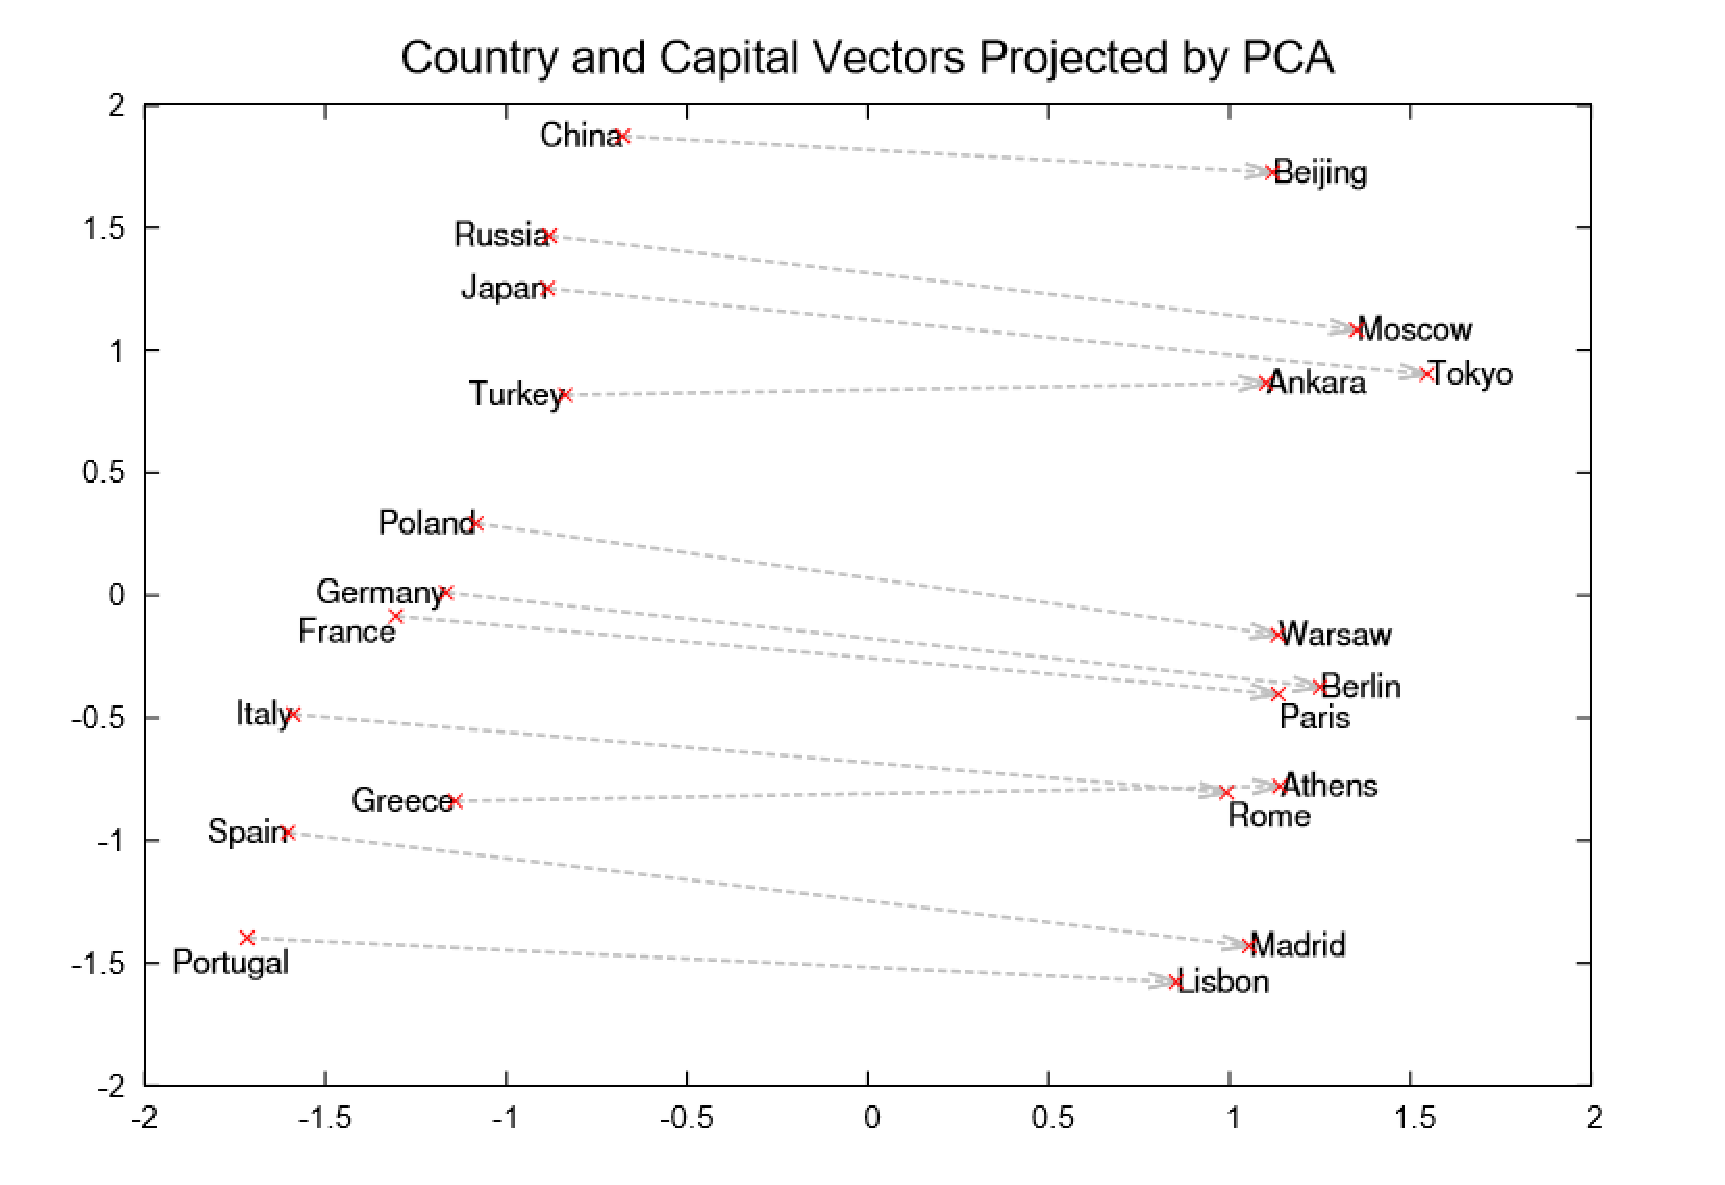
\includegraphics[width=12.5cm]{../images/CCVbyPCAfromM.eps}
  \caption[Country and Capital Vectors Projected by PCA(\cite{drwpc})]{連続Skip-gramモデルで学習した1000次元の単語ベクトルを、主成分分析により2次元に縮約し、いくつかの国名と首都名をプロットしたもの。首都名などの関係情報を与えること無しに、モデルが自動的に単語の概念を暗黙的に学習したことが見て取れる。\cite{drwpc}}
\end{figure}
このグラフにある例を用いて、先ほどと同様に単語集合を作りノードマッチングを行った結果が以下の表(\ref{ccv_c})である
\begin{table}[!h]
  \caption[国名と都市名のマッチング結果]{国名と都市名のマッチング結果}
  \label{ccv_c}
  \begin{center}
    \begin{tabular}{|c||c|} \hline
      集合X & 集合Y \\ \hline \hline
      中国 & 北京 \\
      ポーランド & ワルシャワ \\
      ギリシャ & アテネ \\
      ポルトガル & リスボン \\
      ドイツ & ベルリン \\
      スペイン & マドリード \\
      フランス & パリ \\
      ロシア & モスクワ \\
      トルコ & アンカラ \\
      日本 & 東京 \\
      イタリア & ローマ \\ \hline
    \end{tabular}
  \end{center}
\end{table}
これにより、グラフ(\ref{ccv_pca_m})で確認のできる対応関係と同等のものが抽出できていることがわかった。

グラフ(\ref{ccv_pca_m})\cite{drwpc}において、分散ベクトルの学習モデルは連続Skip-gramモデルで1000次元のベクトルを学習していたのに対し、本実験では学習モデルに連続Bag-of-Wordsモデルを用いて200次元のベクトルを学習していた。ハイパーパラメーターやモデルに差があったが、今回の検証実験により、低次元ベクトルにおいても単語の関係性が反映されていると期待できるので、このまま検証を続けていく。

\section{実験1:着目形態素の近傍形態素でノードマッチング}
次に、入力された単語対それぞれの近傍単語から取得した単語で作成したグループ同士にノードマッチングを適用することで、単語同士の掃除関係が抽出できるかを実験した。

入力した単語対の近傍10個を取得したものが、表()で、この表に対しノードマッチングを適用した結果が、表()である。\\
ここで、近傍の取り方については、着目単語との余弦類似度が高いものを類似度の高さ順に取ってきている。

\begin{table}[!h]
  \begin{minipage}[t]{.45\textwidth}
    \caption[(王,女王)の近傍10単語]{(王,女王)の近傍10単語}
    \label{}
    \begin{center}
      \begin{tabular}{|c||c|} \hline
        集合X & 集合Y \\ \hline \hline
        は王 & 王女 \\
        皇帝 & 王妃 \\
        に王 & 国王 \\
        国王 & エリザベス女王 \\
        君主 & ヴィクトリア \\
        大王 & 王 \\
        王妃 & 王子 \\
        伯 & エリザベス1世 \\
        聖王 & エリザベス2世 \\
        女王 & 王配 \\ \hline
      \end{tabular}
    \end{center}
  \end{minipage}
  \hfill
  \begin{minipage}[t]{.45\textwidth}
    \caption[(王,女王)の近傍10単語でグラフノードマッチング]{(王,女王)の近傍10単語でグラフノードマッチング}
    \label{}
    \begin{center}
      \begin{tabular}{|c||c|} \hline
        集合X & 集合Y \\ \hline \hline
        は王 & 王 \\
        皇帝 & 国王 \\
        女王 & ヴィクトリア \\
        \textbf{国王} & \textbf{エリザベス女王} \\
        に王 & 王妃 \\
        王妃 & 王配 \\
        君主 & 王子 \\
        \textbf{大王} & \textbf{王女} \\
        伯 & エリザベス1世 \\
        \textbf{聖王}\footnote{徳が深い王} & \textbf{エリザベス2世} \\ \hline
      \end{tabular}
    \end{center}
  \end{minipage}
\end{table}

結果を見るに、そもそも形態素解析がうまくできていない部分があったことがわかる。加えて、(王,女王)の関係にあるような対応関係を構築することが、人手でも難しい集合になってしまっていることがわかる。

他の例でもいくつか試してみた。
\begin{table}[!h]
  \begin{minipage}[t]{.45\textwidth}
    \caption[(日本,アメリカ)の近傍10単語]{(日本,アメリカ)の近傍10単語}
    \label{}
    \begin{center}
      \begin{tabular}{|c||c|} \hline
        集合X & 集合Y \\ \hline \hline
        韓国 & 米国 \\
        日本国内 & イギリス \\
        台湾 & 英国 \\
        中国 & カナダ \\
        欧米 & アメリカ合衆国 \\
        海外 & ヨーロッパ \\
        日本の文化 & オーストラリア \\
        日本国外 & フランス \\
        アジア & ドイツ \\
        わが国 & キューバ \\ \hline
      \end{tabular}
    \end{center}
  \end{minipage}
  \hfill
  \begin{minipage}[t]{.45\textwidth}
    \caption[(日本,アメリカ)の近傍10単語でグラフノードマッチング]{(日本,アメリカ)の近傍10単語でグラフノードマッチング}
    \label{}
    \begin{center}
      \begin{tabular}{|c||c|} \hline
        集合X & 集合Y \\ \hline \hline
        韓国 & オーストラリア \\
        欧米 & ヨーロッパ \\
        日本国内 & 米国 \\
        海外 & 英国 \\
        アジア & イギリス \\
        台湾 & キューバ \\
        中国 & ドイツ \\
        日本国外 & カナダ \\
        わが国 & フランス \\
        日本の文化 & アメリカ合衆国 \\ \hline
      \end{tabular}
    \end{center}
  \end{minipage}
\end{table}

\begin{table}[h]
  \begin{minipage}[t]{.45\textwidth}
    \caption[(東京,東京タワー)の近傍10単語]{(東京,東京タワー)の近傍10単語}
    \label{}
    \begin{center}
      \begin{tabular}{|c||c|} \hline
        集合X & 集合Y \\ \hline \hline
        大阪 & 東京スカイツリー \\
        名古屋 & 名古屋テレビ塔 \\
        関西 & スカイツリー \\
        札幌 & 電波塔 \\
        横浜 & 屋上 \\
        京都 & オカンとボクと、時々、オトン \\
        神戸 & ランドマークタワー \\
        静岡 & 六本木ヒルズ \\
        新潟 & タワー \\
        神奈川 & お台場 \\ \hline
      \end{tabular}
    \end{center}
  \end{minipage}
  \hfill
  \begin{minipage}[t]{.45\textwidth}
    \caption[(東京,東京タワー)の近傍10単語のグラフマッチング]{(東京,東京タワー)の近傍10単語のグラフマッチング}
    \label{}
    \begin{center}
      \begin{tabular}{|c||c|} \hline
        集合X & 集合Y \\ \hline \hline
        大阪 & お台場 \\
        札幌 & 六本木ヒルズ \\
        \textbf{名古屋} & \textbf{名古屋テレビ塔} \\
        \textbf{横浜} & \textbf{ランドマークタワー} \\
        新宿 & タワー \\
        関西 & 東京スカイツリー \\
        神奈川 & オカンとボクと、時々、オトン \\
        神戸 & スカイツリー \\
        静岡 & 電波塔 \\
        京都 & 屋上 \\ \hline
      \end{tabular}
    \end{center}
  \end{minipage}
\end{table}

\begin{table}[h]
  \begin{minipage}[t]{.45\textwidth}
    \caption[(北海道,札幌)の近傍10単語]{(北海道,札幌)の近傍10単語}
    \label{}
    \begin{center}
      \begin{tabular}{|c||c|} \hline
        集合X & 集合Y \\ \hline \hline
        道内 & 函館 \\
        札幌 & 小樽 \\
        十勝 & 旭川 \\
        釧路 & 帯広 \\
        東北地方 & 釧路 \\
        十勝支庁 & 札幌市 \\
        道東 & 北海道 \\
        道南 & 仙台 \\
        札幌市 & 新潟 \\
        道北 & 岩見沢 \\ \hline
      \end{tabular}
    \end{center}
  \end{minipage}
  \hfill
  \begin{minipage}[t]{.45\textwidth}
    \caption[(北海道,札幌)の近傍10単語のグラフマッチング]{(北海道,札幌)の近傍10単語のグラフマッチング}
    \label{}
    \begin{center}
      \begin{tabular}{|c||c|} \hline
        集合X & 集合Y \\ \hline \hline
        道内 & 北海道 \\
        釧路 & 釧路 \\
        札幌 & 函館 \\
        \textbf{十勝} & \textbf{帯広} \\
        札幌市 & 岩見沢 \\
        道東 & 旭川 \\
        十勝支庁 & 札幌市 \\
        \textbf{東北地方} & \textbf{仙台} \\
        道南 & 小樽 \\
        道北 & 新潟 \\ \hline
      \end{tabular}
    \end{center}
  \end{minipage}
\end{table}

いくつかのケースを試してみたところ、一組の単語対の近傍単語同士で作ったマッチング10組のうち、与えた単語対の関係と等しいものは平均すると2組程度の取得にとどまった。

正答率の低さの原因として考えられることは、そもそも、与えた単語対の関係を作れる単語が各グループに揃わないことが原因として考えられた。そこから、取得する近傍単語の数を増やし、単語対を作る際のバリエーションを増やせるようにして、再度実験を行った。

\begin{table}[h]
  \begin{minipage}[t]{.45\textwidth}
    \caption[(北海道,札幌)の近傍20単語のグラフマッチング]{(北海道,札幌)の近傍20単語のグラフマッチング}
    \label{}
    \begin{center}
      \begin{tabular}{|c||c|} \hline
        集合X & 集合Y \\ \hline \hline
        道内 & 北海道 \\
        釧路 & 釧路 \\
        札幌市 & 札幌市 \\
        札幌 & 函館 \\
        \textbf{十勝} & \textbf{帯広} \\
        \textbf{青森県} & \textbf{青森} \\
        根室 & 室蘭 \\
        \textbf{道東} & \textbf{北見} \\
        \textbf{九州} & \textbf{福岡} \\
        十勝支庁 & 旭川市 \\ \hline
        釧路市 & 岩見沢 \\
        \textbf{東北地方} & \textbf{仙台} \\
        胆振 & 江別 \\
        函館 & 名古屋 \\
        道南 & 旭川 \\
        空知 & 丘珠 \\
        道北 & 苫小牧 \\
        道外 & 小樽 \\
        留萌 & 新潟 \\
        沖縄県 & 東京 \\ \hline
      \end{tabular}
    \end{center}
  \end{minipage}
  \hfill
  \begin{minipage}[t]{.45\textwidth}
    \caption[(東京,東京タワー)の近傍20単語のグラフマッチング]{(東京,東京タワー)の近傍20単語のグラフマッチング}
    \label{ttt}
    \begin{center}
      \begin{tabular}{|c||c|} \hline
        集合X & 集合Y \\ \hline \hline
        \textbf{大阪} & \textbf{通天閣} \\
        新宿 & サンシャイン60 \\
        名古屋 & お台場 \\
        日比谷 & スカイツリー \\
        関西 & 日本電波塔 \\
        札幌 & 六本木ヒルズ \\
        \textbf{横浜} & \textbf{ランドマークタワー} \\
        赤坂 & 大阪タワー \\
        静岡 & FCGビル \\
        神奈川 & ビル街 \\ \hline
        福岡 & 東京スカイツリー \\
        麹町 & 名古屋テレビ塔 \\
        神戸 & 屋上 \\
        都内 & オカンとボクと、時々、オトン \\
        埼玉 & 電波塔 \\
        京都 & 銀座和光 \\
        愛知 & テレビ塔 \\
        青山 & タワー \\
        渋谷 & 展望台 \\
        金沢 & 鉄塔 \\ \hline
      \end{tabular}
    \end{center}
  \end{minipage}
\end{table}

取得する近傍単語を増やしてノードマッチングを行った結果を確認したが、精度の上昇は見られなかった。原因として、与える単語対が近い位置関係にあり、それぞれの近傍として取得する単語が重複したことにより、同一単語でのマッチングが増え、事実上単語対が消失してしまった。

それ以外のケースにおいては、近傍単語の特徴にばらつきがあることがあげられる。

上記の表(\ref{ttt})においては、(東京,東京タワー)から、(地名,塔などの名所)といった関係の取得を想定していたが、それぞれから取得した近傍単語を見るに、"東京"の近傍には地名が多く出現し、想定通りであったが、"東京タワー"の近傍は"名所"、"塔"、"高所"、"題材とした映画"など、大きくぶれてしまった。これは、元にした"東京タワー"という単語が、名所、シンボル、建造物、イメージなど多岐にわたる意味を含有していたからだと推測される。

また、近傍の取得数が10個の時から出現していた映画タイトルについては、コーパス中の出現回数が31回と、他の単語の出現率の10分の1以下\footnote{鉄塔:570回、東京タワー:610回出現}であり、学習が十分になされなかったためにノイズ的に現れてしまったと認識できる。

\section{実験2:近傍単語をクラスタリングし、クラスター同士のマッチングを見る}
先の実験において、入力した一組の単語対それぞれから得た近傍単語同士のマッチングにより、入力単語対と相似な関係の取得は、近傍単語として取得できる単語の特徴に偏りがあることからよい結果が得られなった。

近傍単語の特徴に偏りがあることを考慮して、取得単語数を増やしてみた場合においても、近傍として設定した領域の重なりや、偏りが解消されないといった問題があった。そこで、偏りを解消するために近傍として取得する単語数を増やし、それぞれで同数のクラスターを作成し、クラスター同士のマッチングを考えた。



\begin{table}[h]
  \begin{minipage}[t]{.45\textwidth}
    \caption["日本"の近傍1000単語を20個のクラスターに分割した様子]{"日本"の近傍1000単語を20個のクラスターに分割した様子}
    \label{}
    \begin{center}
      \begin{tabular}{|c||c|} \hline
        クラスター No. & クラスターの特徴 \\ \hline \hline
        0 & ひらがな(名前) \\
        1 & アジアの国々とその関連  \\
        2 & 文明史など歴史関連語  \\
        3 & 日本史用語類  \\
        4 & ひらがな(意味不明瞭)  \\
        5 & ひらがな(人名) \\
        6 & 人名、日本史用語 \\
        7 & 地理科目系用語 \\
        8 & 国内の地名 \\
        9 & 大学、人名など \\
        10 & 日本-世界に関わる歴史用語 \\ \hline
        11 & 地域、国名 \\
        12 & ひらがな(苗字) \\
        13 & 日系、関連語 \\
        14 & 食 \\
        15 & 地域名、沖縄関連語 \\
        16 & 職業名○○家など \\
        17 & 分野別学者などの肩書 \\
        18 & 団体名、経済用語 \\
        19 & ひらがな(名前) \\ \hline
      \end{tabular}
    \end{center}
  \end{minipage}
  \hfill
  \begin{minipage}[t]{.45\textwidth}
    \caption["アメリカ"の近傍1000単語を20個のクラスターに分割した様子]{"アメリカ"の近傍1000単語を20個のクラスターに分割した様子}
    \label{}
    \begin{center}
      \begin{tabular}{|c||c|} \hline
        クラスター No. & クラスターの特徴 \\ \hline \hline
        0 & 地域、職業名、歴史用語など雑多 \\
        1 & アメリカ関連 人・地名 \\
        2 & 地域名、地理用語 \\
        3 & 商業、政策関連 \\
        4 & アメリカ地域名、問題など \\
        5 & アメリカ系地名 \\
        6 & 地域名、政治 \\
        7 & アメリカ史、人名 \\
        8 & 地名、経済 \\
        9 & 史学系用語 \\
        10 & 州単位の事件など \\ \hline
        11 & 地名、アメリカ国家間問題 \\
        12 & アメリカ系政治用語 \\
        13 & 地名、世界史 \\
        14 & 人権史 \\
        15 & 経済 \\
        16 & 地名 \\
        17 & 政治的世界史用語 \\
        18 & アメリカ-他国間 \\
        19 & 戦争など争い事。 \\ \hline
      \end{tabular}
    \end{center}
  \end{minipage}
\end{table}

\begin{table}[h]
  \caption["日本"のクラスターと"アメリカ"のクラスターの対応関係]{"日本"のクラスターと"アメリカ"のクラスターの対応関係}
  \label{}
  \begin{center}
    \begin{tabular}{|c||c|} \hline
      クラスター No.(日本) & クラスター No.(アメリカ) \\ \hline \hline
      0 & 16 \\
      1 & 17 \\
      2 & 6 \\
      3 & 12 \\
      4 & 2 \\
      5 & 14 \\
      6 & 7 \\
      7 & 3 \\
      8 & 11 \\
      9 & 18 \\ \hline
      10 & 4 \\
      11 & 5 \\
      12 & 19 \\
      13 & 1 \\
      14 & 10 \\
      15 & 8 \\
      16 & 0 \\
      17 & 9 \\
      18 & 15 \\
      19 & 13 \\ \hline
    \end{tabular}
  \end{center}
\end{table}

\begin{table}[h]
  \begin{minipage}[t]{.45\textwidth}
    \caption[]{}
    \label{}
    \begin{center}
      \begin{tabular}{|c||c|} \hline
        集合X & 集合Y \\ \hline \hline
         &  \\
         &  \\
         &  \\
         &  \\
         &  \\
         &  \\
         &  \\
         &  \\
         &  \\
         &  \\ \hline
      \end{tabular}
    \end{center}
  \end{minipage}
  \hfill
  \begin{minipage}[t]{.45\textwidth}
    \caption[]{}
    \label{}
    \begin{center}
      \begin{tabular}{|c||c|} \hline
        集合X & 集合Y \\ \hline \hline
         &  \\
         &  \\
         &  \\
         &  \\
         &  \\
         &  \\
         &  \\
         &  \\
         &  \\
         &  \\ \hline
      \end{tabular}
    \end{center}
  \end{minipage}
\end{table}

この実験を始めるにあたって、まず、近傍単語の様子を確認した。

\begin{table}[h]
  \begin{minipage}[t]{.45\textwidth}
    \caption[(王,女王)]{(王,女王)の近傍単語}
    \label{kq_table}
    \begin{center}
      \begin{tabular}{|c|c|} \hline
        王 & 女王 \\ \hline
        は王 & 王女 \\
        皇帝 & 王妃 \\
        に王 & 国王 \\
        国王 & エリザベス女王 \\
        君主 & ヴィクトリア \\
        大王 & 王 \\
        王妃 & 王子 \\
        伯 & エリザベス1世 \\
        聖王 & エリザベス2世 \\
        女王 & 王配 \\ \hline
      \end{tabular}
    \end{center}
  \end{minipage}
  \hfill
  \begin{minipage}[t]{.45\textwidth}
    \caption[(日本,アメリカ)]{(日本,アメリカ)の近傍単語}
    \begin{center}
      \begin{tabular}{|c|c|} \hline
        日本 & アメリカ \\ \hline
        韓国 & 米国 \\
        日本国内 & イギリス \\
        台湾 & 英国 \\
        中国 & カナダ \\
        欧米 & アメリカ合衆国 \\
        海外 & ヨーロッパ \\
        日本の文化 & オーストラリア \\
        日本国外 & フランス \\
        アジア & ドイツ \\
        わが国 & キューバ \\ \hline
      \end{tabular}
    \end{center}
  \end{minipage}
\end{table}

\newpage

表(\ref{kq_table})に関して、下図にあるような、(男,女)の関係に相当する単語が出力されることを想定していたため、この時点では大きな誤算である。
\begin{figure}[h]
  \centering
  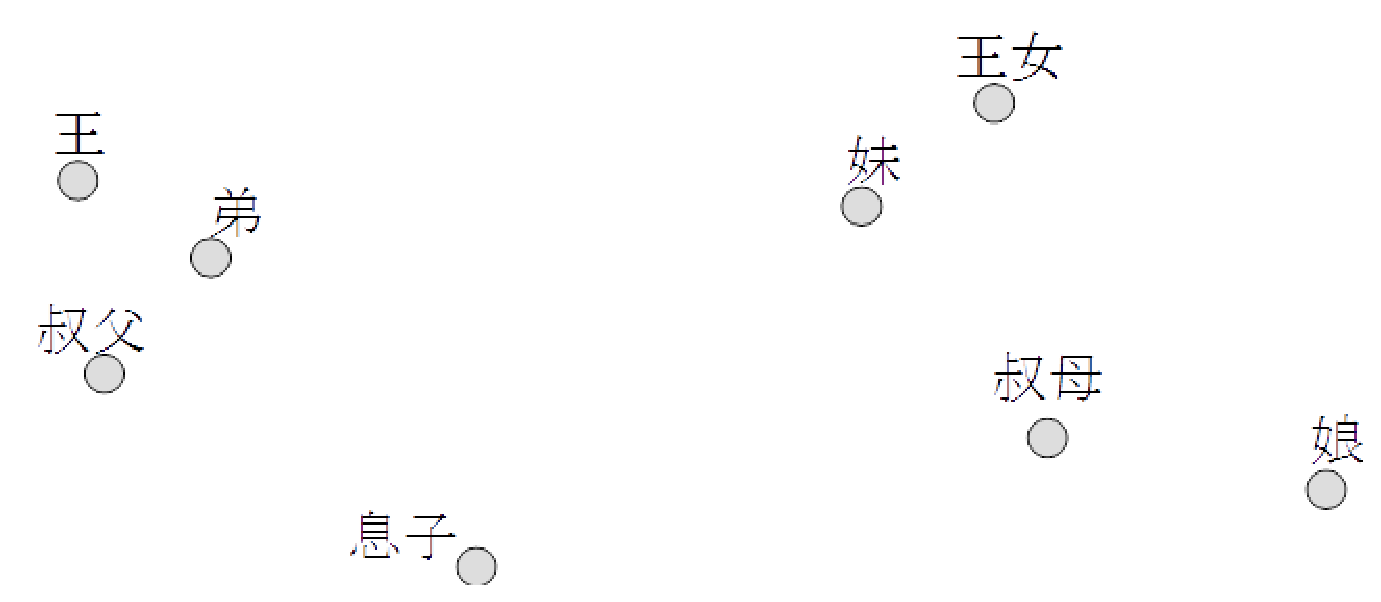
\includegraphics[width=8cm]{../images/kq_fv.eps}
  \caption{王-女王 近傍イメージ}
  \label{kq_fv}
\end{figure}

\begin{table}[h]
  \begin{minipage}[t]{.33\textwidth}
    \caption[(明るい,暗い)]{(明るい,暗い)の近傍単語}
    \begin{center}
      \begin{tabular}{|c|c|} \hline
        暗い & 明るい \\ \hline
        明るく & 暗く \\
        暗く & 明るく \\
        濃い & 薄暗い \\
        淡い & 眩しく \\
        眩しく & 青白い \\
        青白い & 濃い \\
        淡く & 薄暗く \\
        明るめ & 淡い \\
        鮮やか & ぼんやり \\ \hline
      \end{tabular}
    \end{center}
  \end{minipage}
  \begin{minipage}[t]{.66\textwidth}
    \caption[(光,影,闇)]{(光,影,闇)の近傍単語}
    \begin{center}
      \begin{tabular}{|c|c|c|} \hline
        太陽光 & 影の & 暗黒 \\ \hline
        反射 & 闇 & 妖魔 \\
        発光 & 暗闇 & 魔物 \\
        光線 & 暗部 & 邪悪 \\
        鏡 & 影 & 魔神 \\
        光源 & 暗い & 影 \\
        紫外線 & 隠れ & 悪魔 \\
        い光 & 暗黒 & 魔王 \\
        透かす & 其面 & 魔界 \\
        太陽 & 潜む & 魔 \\ \hline
      \end{tabular}
    \end{center}
  \end{minipage}
\end{table}
以上の結果を見るに、単純に近傍単語を同数取ってきたグループで作成するグラフは、与えた単語対が持つ関係を保持した同型のグラフには必ずしもなっていないことが予想される。
